% Generated by paper/figures/src/v6_baseline_deltas.py from results/a4k195_main_sca_v2 and results/a4k195_main
% (paired per-image differences through v2swap.derived_pairs, checked against the summaries); do not edit by hand.
\begin{figure}[!htbp]
  \centering
  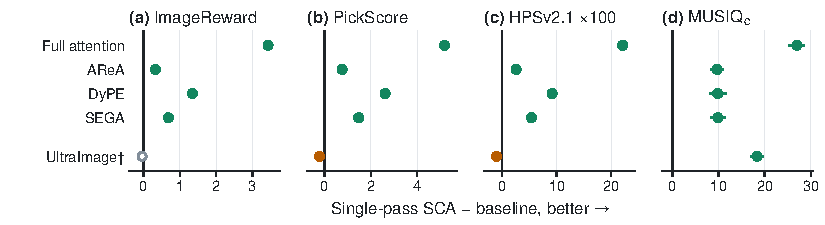
\includegraphics[width=\linewidth]{figures/v6/baseline_deltas.pdf}
  \caption{\textbf{Single-pass \sca{} beats every shared-sampler baseline on all four metrics; against UltraImage the result is mixed.}
  Single-pass \sca{} minus each baseline on the same 195 prompts at $4096^2$, seed 0; whiskers are 95\% paired intervals over prompts (2000 bootstrap draws), not adjusted for multiplicity. Filled: the interval excludes zero (green: \sca{} better, orange: worse); open grey: it includes zero.
  Against UltraImage, \sca{} is better on MUSIQ$_\text{c}$ and worse on PickScore and HPSv2.1; $^\dagger$UltraImage runs its own two-stage recipe, so this is not an equal-cost comparison. Table~\ref{tab:panel46_deltas} gives all metrics.}
  \label{fig:baseline_quality}
\end{figure}
